\documentclass[aspectratio=169]{beamer}
\usetheme[background=light]{metropolis}

\usepackage[utf8]{inputenc}
\usepackage[T1]{fontenc}
\usepackage[verbose]{placeins}
\usepackage{color}
\usepackage{caption}
\usepackage{subcaption}

\usepackage{marvosym}
\usepackage[marvosym]{tikzsymbols}

\title{An introduction to Docker, WIP\\\small{chroot on steroids}}
\date{25th June, 2019}
\author{Patrick Schiffler}
\institute{}
\begin{document}
	\maketitle
	
	\section{Chapter 1: Let us spread a new technology.}
	
	\begin{frame}{Motivation}
		Virtual Machines are old fashioned and complete garbage. \Vomey[2]
	\end{frame}
	
	\begin{frame}{Motivation}
		Guys, chill. \Cooley[2]
	\end{frame}
	
	\begin{frame}{Motivation}
		In reality, we need technologies which fit better into the cloud concept.
	\end{frame}
	
	\section{Chapter 2: The answer is Containers}
	
	\begin{frame}[allowframebreaks]{Characteristics}
		What does docker.com say about containers?\\
		Containers are ...
		\begin{itemize}
			\item flexible
		  	\item lightweight
		  	\item interchangeable
		  	\item portable
		  	\item scalable
		  	\item stackable
	  	\end{itemize}
		\framebreak
		But people always say: \emph{Containers are stateless and that's a problem!}\\
		\vspace{5em}
		\dots the f**k?
		\framebreak
		\\Container are primary stateless, and that gives us:
		\begin{itemize}
			\item Reliability
			\item Reproducibility (science loves it)
			\item \dots (probably a lot more)
		\end{itemize}
  	\end{frame}


	\begin{frame}{Container vs. VM}
	    \begin{figure}
			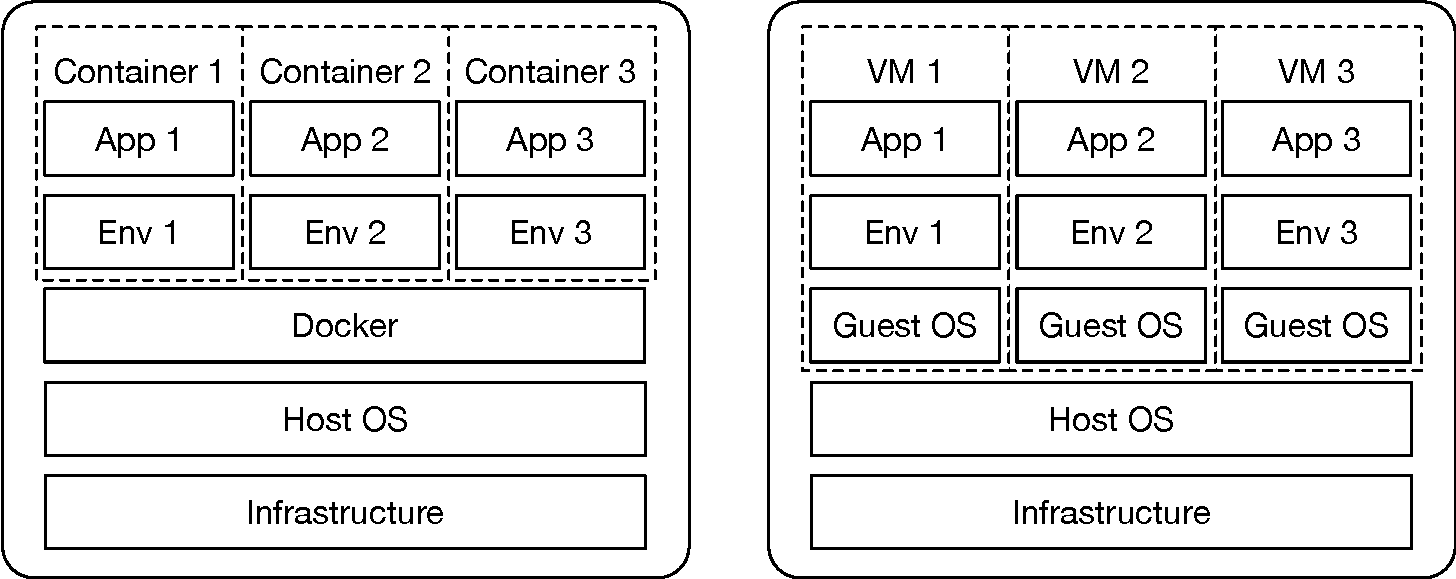
\includegraphics[width=0.8\textwidth]{./assets/container_vm.pdf}
	    \end{figure}
	\end{frame}

	\section{Chapter 3: Sounds good, any volunteers?\newline Docker}

	\begin{frame}[allowframebreaks]{Docker}
		\begin{itemize}
			\item Started in 2013
			\item Implementation of container execution
			\item Client/Server
			\item written in Go
		\end{itemize}
		\framebreak
		Commands
		\begin{itemize}
			\item \texttt{docker run}
			\item \texttt{docker images}
			\item \texttt{docker build}
			\item \texttt{docker exec}
			\item \texttt{docker info / docker inspect}
			\item \texttt{docker logs}
			\item \texttt{docker ps}
			\item \dots
		\end{itemize}
	\end{frame}

	\begin{frame}[allowframebreaks]{Dockerfile $\rightarrow$ Image $\rightarrow$ Container}
		\begin{itemize}
			\item Dockerfile: Blueprint for image
			\item[] $\rightarrow$ Image build from Dockerfile
			\item Image: template for container
			\item[] $\rightarrow$ Container is instance of image $\rightarrow$ A running Image
		\end{itemize}
		\framebreak
		Directives
		\begin{itemize}
			\item \texttt{FROM}
			\item \texttt{MAINTAINER (deprecated appereantly)}
			\item \texttt{RUN}
			\item \texttt{COPY}
			\item \texttt{CMD}
			\item \texttt{ENTRYPOINT}
			\item \dots
		\end{itemize}
	\end{frame}

	\begin{frame}{Images}
		Encapsulate the\dots
		\begin{itemize}
			\item application
			\item runtime environment
			\item all installable data to run an application
		\end{itemize}
		\framebreak
		Images are\dots
		\begin{itemize}
			\item prebuilt or custom
			\item stored locally or in a registry
			\item tagged
			\item build up in layers
		\end{itemize}
	\end{frame}

	\begin{frame}{Docker Hub}
		\begin{itemize}
			\item hub.docker.com
			\item Default registry
			\item Free to use (open repos)
		\end{itemize}
	\end{frame}

	\begin{frame}{Docker container}
		\begin{itemize}
			\item Running Image
			\item Executes command/entrypoint
			\item Dies automatically
		\end{itemize}
	\end{frame}

	\section{Chapter 4: Let's see it in action}

	%HIER GEHTS WEITER

	\begin{frame}{Monitoring approach(ish)}
		\begin{itemize}
			\item Sharing the host kernel $\rightarrow$ Processes visible in host system
			\item Processes in container run as \texttt{root} (by default)
			\item Dockerfile $\rightarrow$ USER
		\end{itemize}
	\end{frame}

	\begin{frame}{Disadvantages, from my personal pov}
		\begin{itemize}
			\item We still need to learn a new technology
			\item No cross-platform (don't even think about qemu)
			\item Open-source (yes, sorry) $\rightarrow$ You never know where it's leading to
		\end{itemize}
	\end{frame}

	\section{Outlook}
	\begin{frame}{Orchestration}
		\begin{itemize}
			\item Docker swarm
			\item Kubernetes
			\item Google Cloud
			\item AWS
			\item Azure
		\end{itemize}
	\end{frame}

	\section{Thanks for your attention!}
	
	\begin{frame}{Wow}
	    \begin{figure}
	  		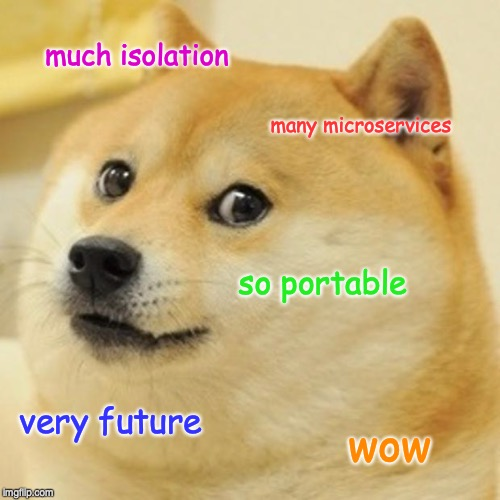
\includegraphics[width=0.9\textheight]{./assets/wow.jpg}
	    \end{figure}
	\end{frame}
	
	\section{Questions?}
	
\end{document}
